\documentclass[review]{elsarticle}
\usepackage{hyperref}
\usepackage[margin=1in]{geometry}
\usepackage{graphicx}
\usepackage{amsmath}
\usepackage{placeins}
\usepackage{comment}
\usepackage{gensymb}
\usepackage{lineno}
\usepackage{comment}
\usepackage{color}

\journal{Journal of Nuclear Materials}
\bibliographystyle{elsarticle-num}

\begin{document}

\begin{frontmatter}
\title{Atomistic calculations of the surface energy as a function of composition and temperature in $\gamma$ U-Zr to inform fuel performance modeling}


\author[inl,ncsu]{Benjamin Beeler\corref{qwe}}
\cortext[qwe]{Corresponding author}
\ead{benjamin.beeler@inl.gov}
\author[inl]{Albert Casagranda}
\author[inl]{Larry Aagesen}
\author[inl]{Yongfeng Zhang}
\author[inl]{Stephen Novascone}
\address[inl]{Idaho National Laboratory, Idaho Falls, ID 83415}
\address[ncsu]{North Carolina State University, Raleigh, NC 27607}


\begin{abstract}

Uranium-zirconium alloy fuels are candidates for advanced sodium cooled fast reactors, due to their high uranium density, high thermal conductivity, inherent safety and ability to incorporate minor actinides into the fuel. Unlike traditional ceramic UO$_2$ fuel, U-Zr alloys swell rapidly and substantially, but the actual mechanistic process of swelling, including the rate of swelling, is not well understood. Fuel performance models are being developed to describe the swelling process, but these models currently lack the requisite underlying physics and fundamental property data to be truly predictive. In this work, molecular dynamics simulations are utilized to investigate a number of bulk thermophysical properties in  $\gamma$U-Zr, the void surface energy as a function of temperature and composition, and the void free energy. Finally, the effect of surface energy on fuel swelling behavior is demonstrated via finite element based fuel performance simulations, emphasizing the importance of the inclusion of accurate fundamental material properties. 


\end{abstract}
\end{frontmatter}

\linenumbers
\modulolinenumbers[5]

\section{Introduction}

Uranium-zirconium (U-Zr) and uranium-plutonium-zirconium (U-Pu-Zr) alloy fuels have a history of usage in sodium-cooled fast reactors. Due to the excellent neutron economy and high burnup capability, metallic fuel has a successful track record in sodium-cooled fast reactors such as EBR-II \cite{hofman1997}. Recently, U-Zr fuels have regained interest due to the possibility of incorporating minor actinides into the fuel, and as such the metallic fuel alloys would serve to reduce the quantity of long-lived radioisotopes generated as nuclear waste \cite{capriotti2017}. Additionally, in February 2019, the U.S. Department of Energy announced its plans to build a Versatile Test Reactor, or VTR, which will utilize metallic fuel. 

Historically, U-Zr alloys were typically employed as a cylindrical fuel rod surrounded by cladding \cite{ogata2012}, similar to UO$_{2}$ fuels. Unlike UO$_{2}$ fuels, dramatic swelling is inevitable, and is typically accounted for by manufacturing fuels with a smear density of approximately 75{\%}. This allows for approximately 30\% swelling, which is sufficient to allow for porosity interconnection and fission gas release \cite{beck1968}. Irradiation experiments were typically focused on the total amount of swelling, since the target was achieving very high burnup in these fuels \cite{hofman1997}. However, as alternate fuel geometries are potentially being pursued and there is interest in utilizing these fuel alloys at low burnup and high smear density, the actual mechanistic process of swelling, including the rate of swelling, needs to be understood. 

The nature of swelling is anisotropic in these fuels, largely due to the difference in swelling behavior between the hotter center of the fuel and the colder periphery \cite{hofman1990}. During operation, the phenomenon of constituent redistribution takes place. This results in three distinct radial phase regions within the fuel. The innermost region is Zr-enriched, the intermediate region is Zr-depleted and the outermost region has a nominal Zr concentration. This phenomenon is due to both the effect of the temperature gradient on phase equilibria and the diffusion of species along the temperature gradient both radially and axially. This concentration variance as a function of radius in combination with the temperature gradient leads to the $\gamma$ phase being present in the interior of the fuel pellet, while the $\alpha$ phase dominates the periphery \cite{kobayashi1990, kim2004}. 

The $\gamma$ phase of U-Zr typically presents large fission gas bubbles and as such is of primary interest when analyzing fission gas induced swelling in U-Zr. However, there is limited fundamental property data on the $\gamma$ phase, largely due to its low temperature thermodynamic and mechanical instability, which inhibits both experimental and computational study. The historical experimental thermophysical data is nicely summarized in part 1 of the metallic fuels handbook \cite{handbook1}, which includes phase diagrams, heat capacities, thermal expansion and thermal conductivities. However, there are discrepancies between diffraction and transmission electron microscopy studies on the nature of the phase compositions and phase transformations. Calorimetry, thermal expansion and mechanical properties data can be highly dependent upon oxygen, carbon and nitrogen impurity content. Generally few experiments were conducted for each individual property and results are susceptible to experimental uncertainties \cite{janney2018}. The computational literature on U-Zr alloys is even more scarce, where the totality of research on $\gamma$ U-Zr is an individual study of point defects via density functional theory methods \cite{beeler2010} and an interatomic potential that was developed that can accurately describe a number of thermophysical properties in $\gamma$ U-Zr \cite{moore2015}. 

One key fundamental property that is of particular interest to fuel performance and mesoscale models of fission gas swelling is the surface energy, of which there is no prior experimental or computational information. The surface energy controls bubble morphology and evolution and can dramatically impact fuel swelling kinetics due to fission gas bubbles.  In this paper, molecular dynamics simulations have been performed to calculate a number of bulk thermophysical properties of $\gamma$U-Zr alloys, with an emphasis on the void surface energy, from 900 K to 1300 K. This work is incorporated into fuel performance simulations to demonstrate the impact on fission gas swelling predictions in U-Zr fuels.

\section{Computational Details}

Molecular dynamics simulations are performed utilizing the LAMMPS \cite{plimpton1995} software package and the U-Zr MEAM interatomic potential from Moore, et al. \cite{moore2015}. It should be emphasized that the results from Moore \cite{moore2015} utilized the DYNAMO code \cite{dynamo}, and while it was a precursor to LAMMPS, it has slightly different implementations, and thus verification of bulk properties is critical to ensuring both a functioning potential and accuracy of results. 

For the generation of equilibrium properties, a 10x10x10 supercell with 2000 atoms and periodic boundaries is generated with a prescribed chemical composition ranging from pure body-centered cubic (bcc) U to pure bcc Zr, with eleven unique alloy compositions. Alloys of U-Zr are generated by constructing a bcc U system, with a prescribed number of U atoms replaced by Zr. Relaxation is performed in an NPT-ensemble with a Nose-Hoover barostat and thermostat, relaxing each x, y, and z component individually with a damping parameter of 0.1 for both the barostat and thermostat. Systems are investigated from 900 K up to 1400 K, in increments of 100 K. One hundred unique simulations are performed for each system, unique with respect to compositional configuration, to ensure statistical significance of the results.

The formation energy per atom is determined by equation \ref{eq1}

\begin{equation}
\label{eq1}
E_{f}/at= \frac{E(UZr) - E(U)\times N(U) - E(Zr)\times N(Zr)}{N}
\end{equation} where E(UZr) is the total energy of the system of interest, E(U) is the energy per atom of bcc U, N(U) is the number of U atoms in the system, E(Zr) is the energy per atom of bcc Zr, N(Zr) is the number of Zr atoms in the system and N is the total number of atoms in the system. The coefficient of thermal expansion is calculated by equation \ref{eq2}

\begin{equation}
\label{eq2}
\alpha= \frac{(\frac{V_2}{V_1})^{1/3} - 1}{T_2-T_1}
\end{equation} where V$_2$ and V$_1$ are the volumes at temperatures T$_2$ and T$_1$. The heat capacity is determined from equation \ref{eq3}

\begin{equation}
\label{eq3}
C_p= \frac{TE_2 - TE_1}{T_2-T_1} 
\end{equation} where TE$_2$ and TE$_1$ are the total energies of the system at T$_2$ and T$_1$. 

The interval T$_1$ to T$_2$ is sufficiently small to make the assumption that the coefficient of thermal expansion and the heat capacity are constant in this temperature range. One methodology for determining an average surface energy is to investigate the surface energy of a void. This approximates a system with a number of planar surfaces, while allowing the void surface to reorient to low energy planes, providing a more realistic surface configuration than can be obtained by investigating a set of planar surfaces. For the calculation of void surface energies, a 30x30x30 supercell with 54,000 atoms was generated with periodic boundaries at a given chemical composition. Utilizing the same NPT-ensemble details as for equilibrium properties, the system is equilibrated for 50 ps. Subsequently, atoms within a spherical region of a prescribed size are removed from the center of the supercell, generating a void, and the system is allowed to relax for a further 50 ps. Averaging of the system potential energy is performed over the final 25 ps of each individual 50 ps segment. The surface energy is calculated via equation \ref{eq:surface},

\begin{equation}
\label{eq:surface}
E_{surf}= \frac{(E^{*} - E)}{A} \times N
\end{equation} where $\it{E^{*}}$ is the potential energy per atom of the system with a void, $\it{E}$ is the potential energy per atom of the perfect crystal U, Zr or U-Zr, $\it{A}$ is the total surface area of the void and $\textit{N}$ is the number of atoms in the system with a void. Five unique systems are investigated for each temperature, composition and void size.

The reduction of the free energy of the system determines the manner in which the microstructure of a given system evolves. Thus, in addition to obtaining surface energies, it is valuable to investigate the entropy of systems containing voids as well. The change in entropy of the system is determined by equation \ref{eq:entropy},

\begin{equation}
\label{eq:entropy}
\Delta S = \int_{T_{1}}^{T_{2}} \frac{C_{p}}{T} dT
\end{equation}

where C$_{p}$ is the constant pressure heat capacity in the temperature range T$_{1}$ to T$_{2}$. By integrating, the change in entropy can be evaluated as:

\begin{equation}
\label{eq:entropy2}
\Delta S = C_{p} \times (ln(T_{2}) - ln(T_{1})) 
\end{equation}

The heat capacity is determined by the centered-finite difference approach in equation \ref{eq:cp},

\begin{equation}
\label{eq:cp}
C_{p} = \frac{(E_{2} - E_{1})}{(T_{2} - T_{1})} 
\end{equation}

where \textit{E} is the total energy (potential + kinetic) of the system at a given temperature T. This formalism makes use of the assumption that C$_{p}$ is constant over the T$_{1}$ to T$_{2}$ temperature range. To ensure that only the void contribution to the entropy change is being evaluated, the entropy change induced by the bulk is subtracted from the total entropy change of the system with a void. Additionally, the entropy change is divided by the void surface area. This is identical to calculating the entropies from void surface energies, which can be shown by equation \ref{eq:entropy_alt}:

\begin{equation}
\label{eq:entropy_alt}
\Delta S =\frac{ E_{surf}^{T_2} - E_{surf}^{T_1}}{T_2 - T_1} \times [ ln(T_2) - ln(T_1) ]
\end{equation}

where E$_{surf}^{T_{x}}$ is the surface energy from equation \ref{eq:surface} at a given temperature T$_x$. Either equations \ref{eq:entropy}, \ref{eq:entropy2} and \ref{eq:cp} or equation \ref{eq:entropy_alt} can be utilized to calculate the entropy change associated with a void, with identical results. 

Finally, the free energy change is determined by equation \ref{eq:free}:

\begin{equation}
\label{eq:free}
\Delta G = \Delta U - T \Delta S
\end{equation}

where $\Delta S$ is taken from equation \ref{eq:entropy_alt} and $\Delta U$ is the change in internal energy (identical to enthalpy when P=0, as is the case in these systems) of the system. Similar to entropy, to ensure that only the void contribution to the enthalpy change is being evaluated, the enthalpy change induced by the bulk is subtracted from the total enthalpy change of the system with a void.


\section{Results}
\subsection{Equilibrium properties of $\gamma$-UZr}\label{sec:res1}

The energy per atom, formation energy per atom and equilibrium volume per atom, as a function of Zr composition, are shown in Fig. \ref{fig:Eperat}, Fig. \ref{fig:Efperat} and Fig. \ref{fig:Vperat}, respectively. 

The energy per atom decreases monotonically as a function of Zr content, while increasing as a function of temperature for all compositions investigated. This is due to the reference state cohesive energies for U and Zr. The formation energy displays a very unique behavior as a function of composition, showing an initial increase with small additions of Zr. Below 15 atomic percent, the formation energy is positive, while above 15 atomic percent, the formation energy is negative. The formation energy reaches a minimum around 60 atomic percent Zr. This is in agreement with previous computational and experimental studies \cite{moore2015}. Interestingly, there is effectively no variance of the formation energy per atom as a function of temperature. It should be emphasized that only the potential energy of the system is included in this investigation. The volume per atom increases monotonically with increasing Zr content. The change in volume as a function of temperature is more significant for low Zr content alloys, indicating a higher thermal expansion for U-rich U-Zr alloys than for Zr-rich U-Zr alloys at high temperature. 

\begin{figure}[!htp]
\begin{center}
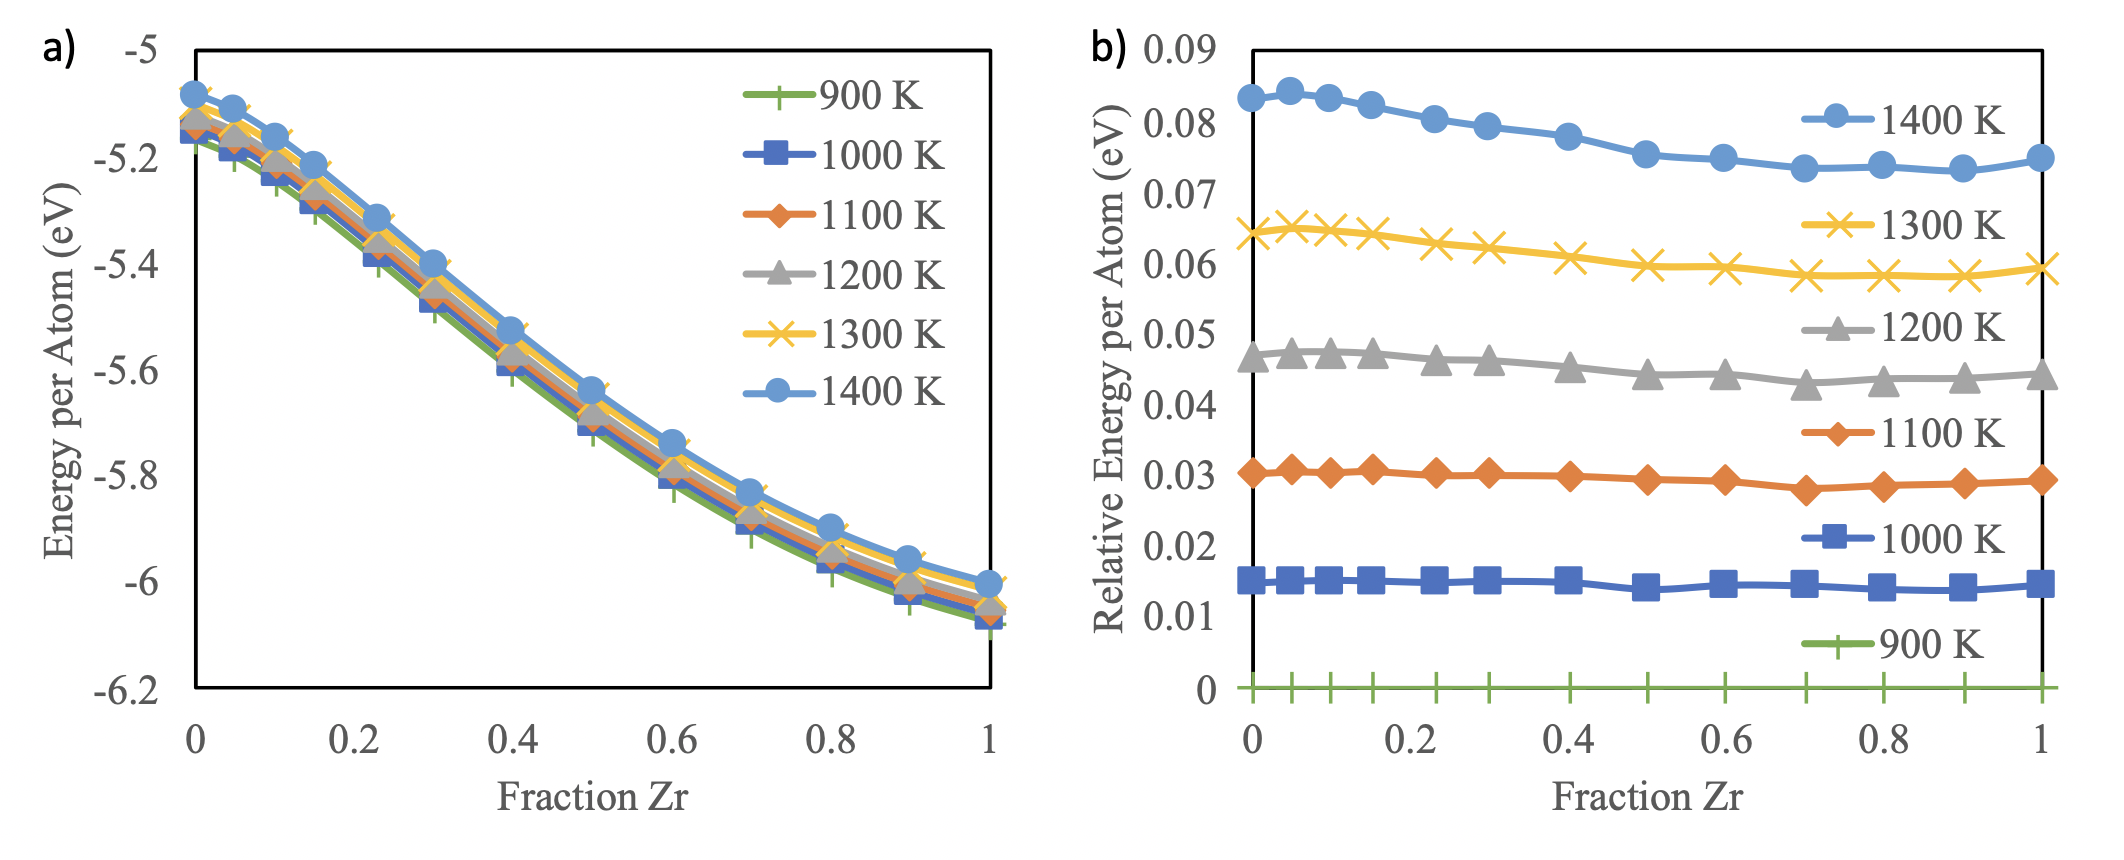
\includegraphics[width=0.6\textwidth]{1_Eperat}
\end{center}
\caption{Energy per atom as a function of Zr content from 900 K to 1400 K. }
\label{fig:Eperat}
\end{figure}

\begin{figure}[!htp]
\begin{center}
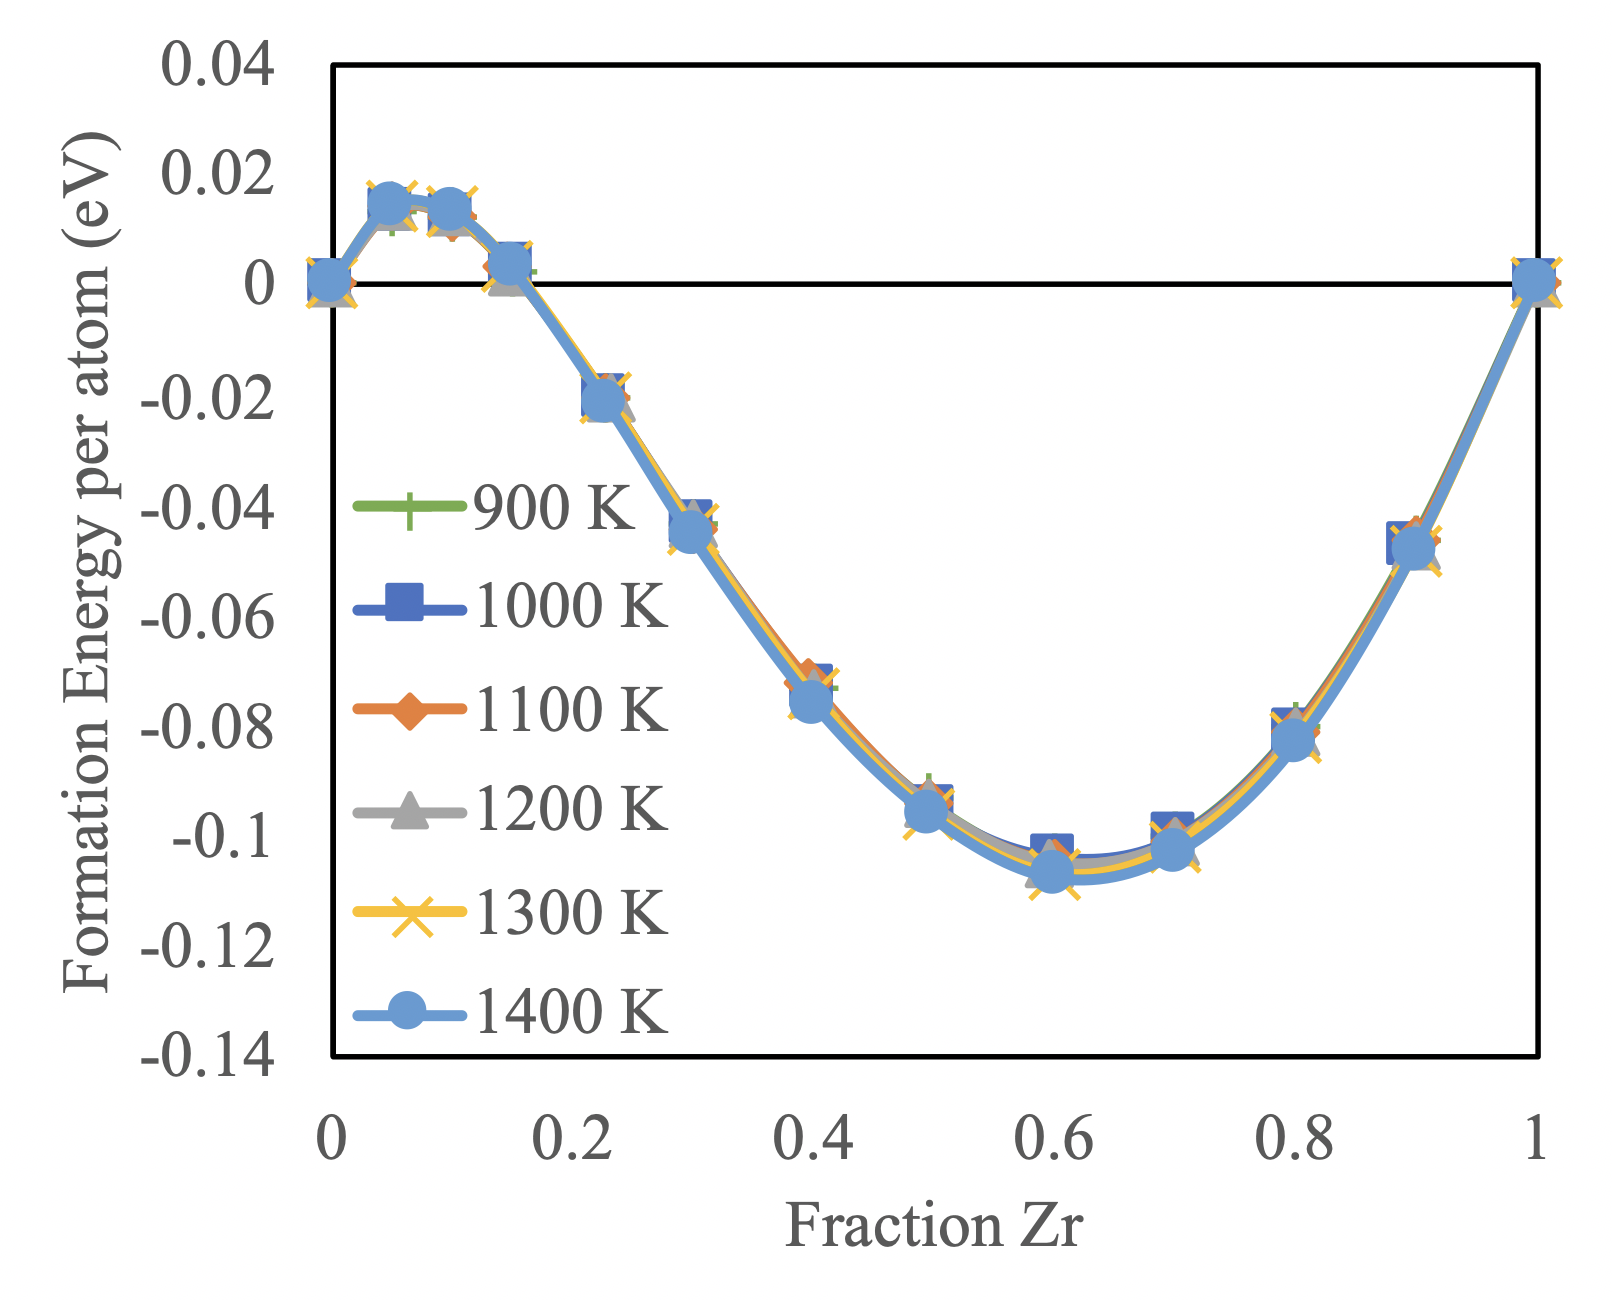
\includegraphics[width=0.6\textwidth]{2_Efperat}
\end{center}
\caption{Formation energy per atom as a function of Zr content from 900 K to 1400 K.  }
\label{fig:Efperat}
\end{figure}

\begin{figure}[!htp]
\begin{center}
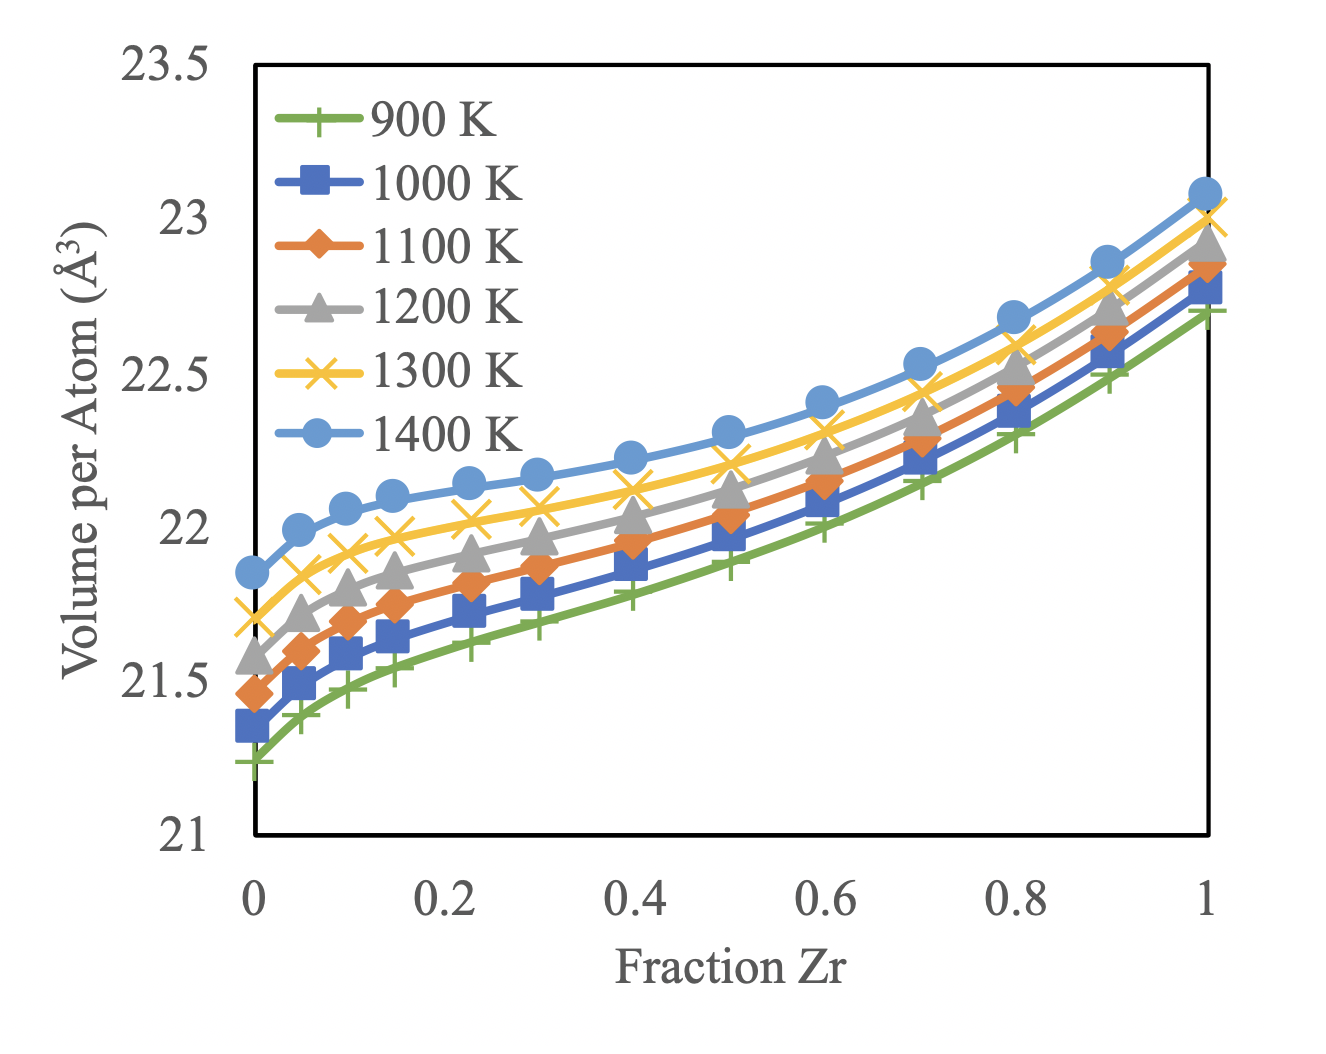
\includegraphics[width=0.6\textwidth]{3_Vperat}
\end{center}
\caption{Volume per atom as a function of Zr content from 900 K to 1400 K.  }
\label{fig:Vperat}
\end{figure}

\FloatBarrier

Given this data, thermal expansion and heat capacity as a function of temperature and composition can be determined, which are shown in Fig. \ref{fig:Texp} and \ref{fig:cp}. The thermal expansion is determined from equation \ref{eq2}. To construct a value at 950 K, the data at 900 K and 1000 K is utilized, thus the midpoint of the data set is the label and this work assumes that the thermal expansion is constant over this temperature interval. This same temperature construction and assumptions on heat capacity are also applied in Fig. \ref{fig:cp}. It can be seen that there does exist a near monotonic trend of decreasing thermal expansion with increasing Zr content, where the coefficient of thermal expansion for bcc U is 1.6 times higher than for bcc Zr at 1050 K. It can also be observed that with increasing temperature, there is a slight increase in the thermal expansion coefficient, with that increase being more prevalent for bcc U than for bcc Zr. Comparing to experimental data at 1200 K from Basak \cite{basak2009} for a U-10Zr alloy (10 weight percent), this interatomic potential predicts a thermal expansion of 1.5E-5, while Basak determined the value to be 1.7E-5, which is quite good agreement. The heat capacity is determined from equation \ref{eq3} and is calculated at each temperature and composition.  There is substantial scatter in the dataset, as would be expected. Both contributions from high temperature thermal fluctuations and localized variations in composition lead to small changes in the energy of the system which are in turn reflected in the heat capacity calculations. The statistical noise may be reduced slightly by simulating for longer times, but the main component of the noise is due to configurational randomness, which is only reduced by simulating many more systems. Regardless, trends do exist of a slight decrease in the heat capacity with increasing Zr content and a slight increase with increasing temperature. The variation with temperature is again more prevalent for bcc U than for bcc Zr. Experimental results show that there is limited variance in the heat capacity with temperature for bcc U-Zr alloys and that the magnitude of the heat capacity tends to decrease slightly with increasing Zr content, which corresponds with these simulation results. However the range in the heat capacity across Zr compositions is from the mid- to low-30s in J/mol-K \cite{janney2018}, which is slightly higher than the values predicted by the interatomic potential in this work. However, as Moore showed \cite{moore2015}, including effects for electronic heat capacity shows that these results compare incredibly well with the experimental literature. 

\begin{figure}[!htp]
\begin{center}
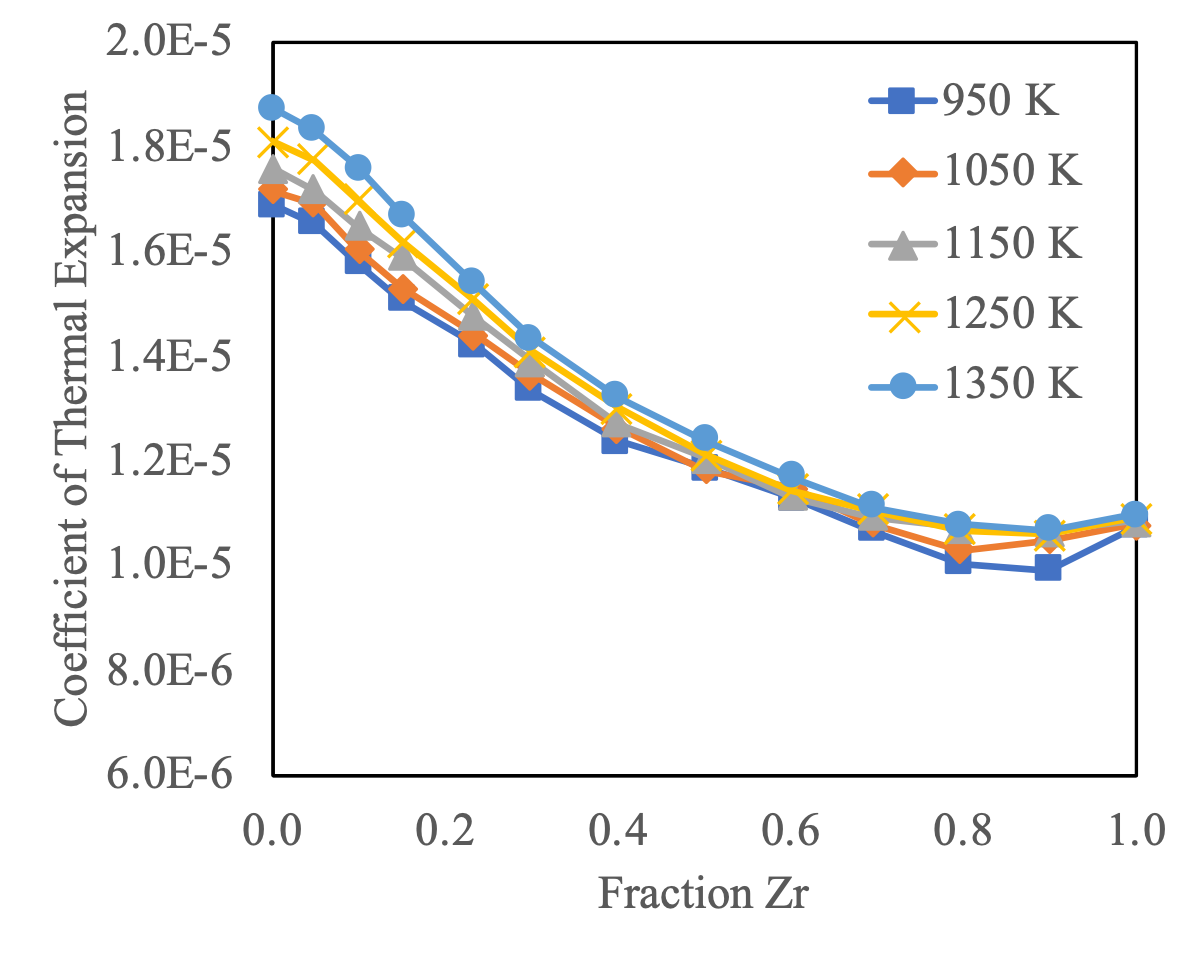
\includegraphics[width=0.6\textwidth]{4_Texp}
\end{center}
\caption{Calculated coefficient of thermal expansion for $\gamma$U-Zr from 900 K to 1400 K as a function of Zr composition.  }
\label{fig:Texp}
\end{figure}


\begin{figure}[!htp]
\begin{center}
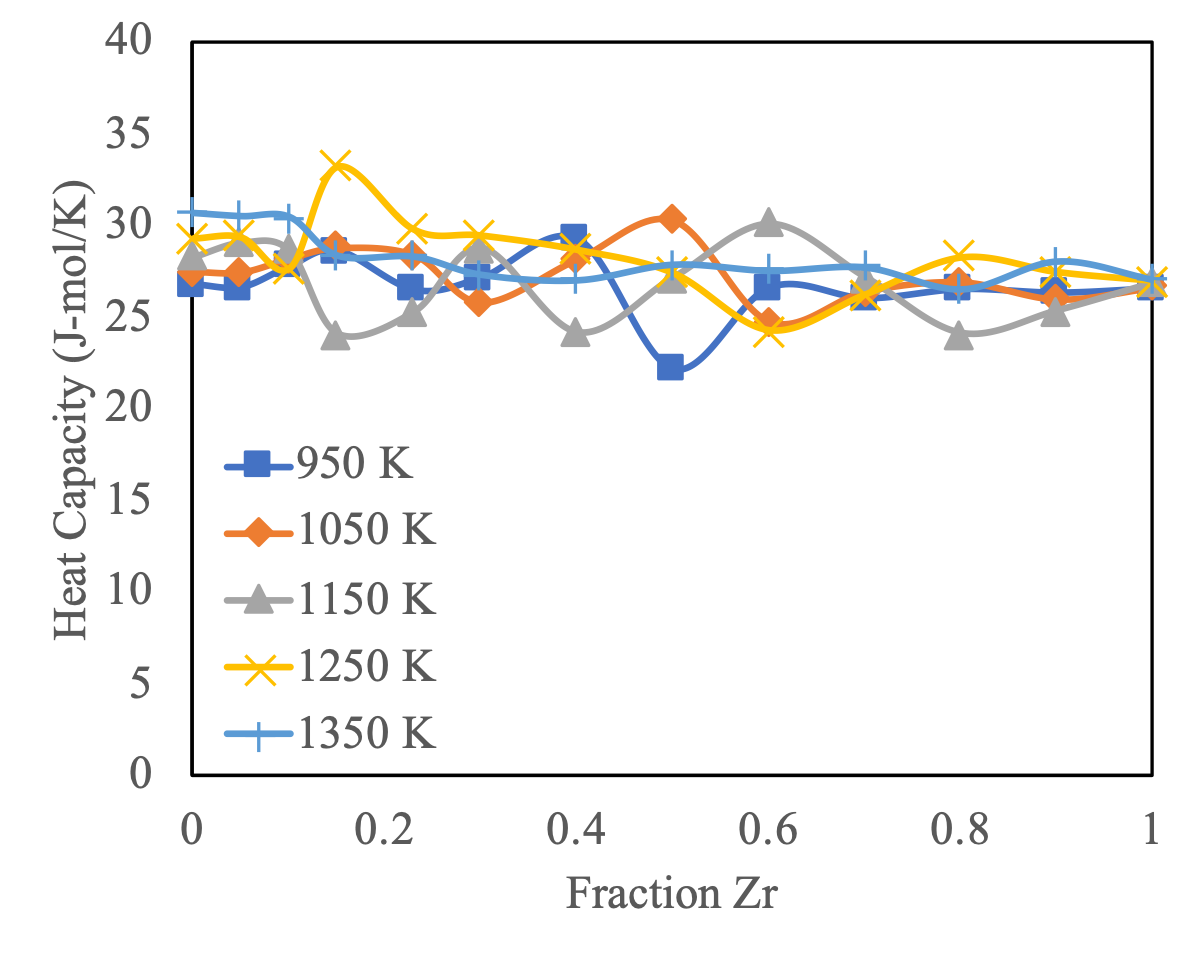
\includegraphics[width=0.6\textwidth]{5_Cp}
\end{center}
\caption{The calculated molar heat capacity for $\gamma$U-Zr from 900 K to 1400 K as a function of Zr composition. }
\label{fig:cp}
\end{figure}

\FloatBarrier

\subsection{Investigation of void surface energy and free energy}\label{sec:res2}

The void surface energy at 1000 K for a U-10Zr alloy as a function of void size is shown in Fig. \ref{fig:size}. As void size increases, the surface energy increases and converges to a given value. For small voids, the curvature of the void surface is relatively high, and as such atoms along the surface are still able to interact with a number of atoms that are also along the surface of the void. This approximates a pseudo-void state that is intermediate between an atom being in the bulk and an atom on a free planar surface, hence the lower surface energy of small voids. To ensure that the surface energy in large voids is being calculated, only voids with a radius of 25 {\AA} are investigated further. 

\begin{figure}[!htp]
\begin{center}
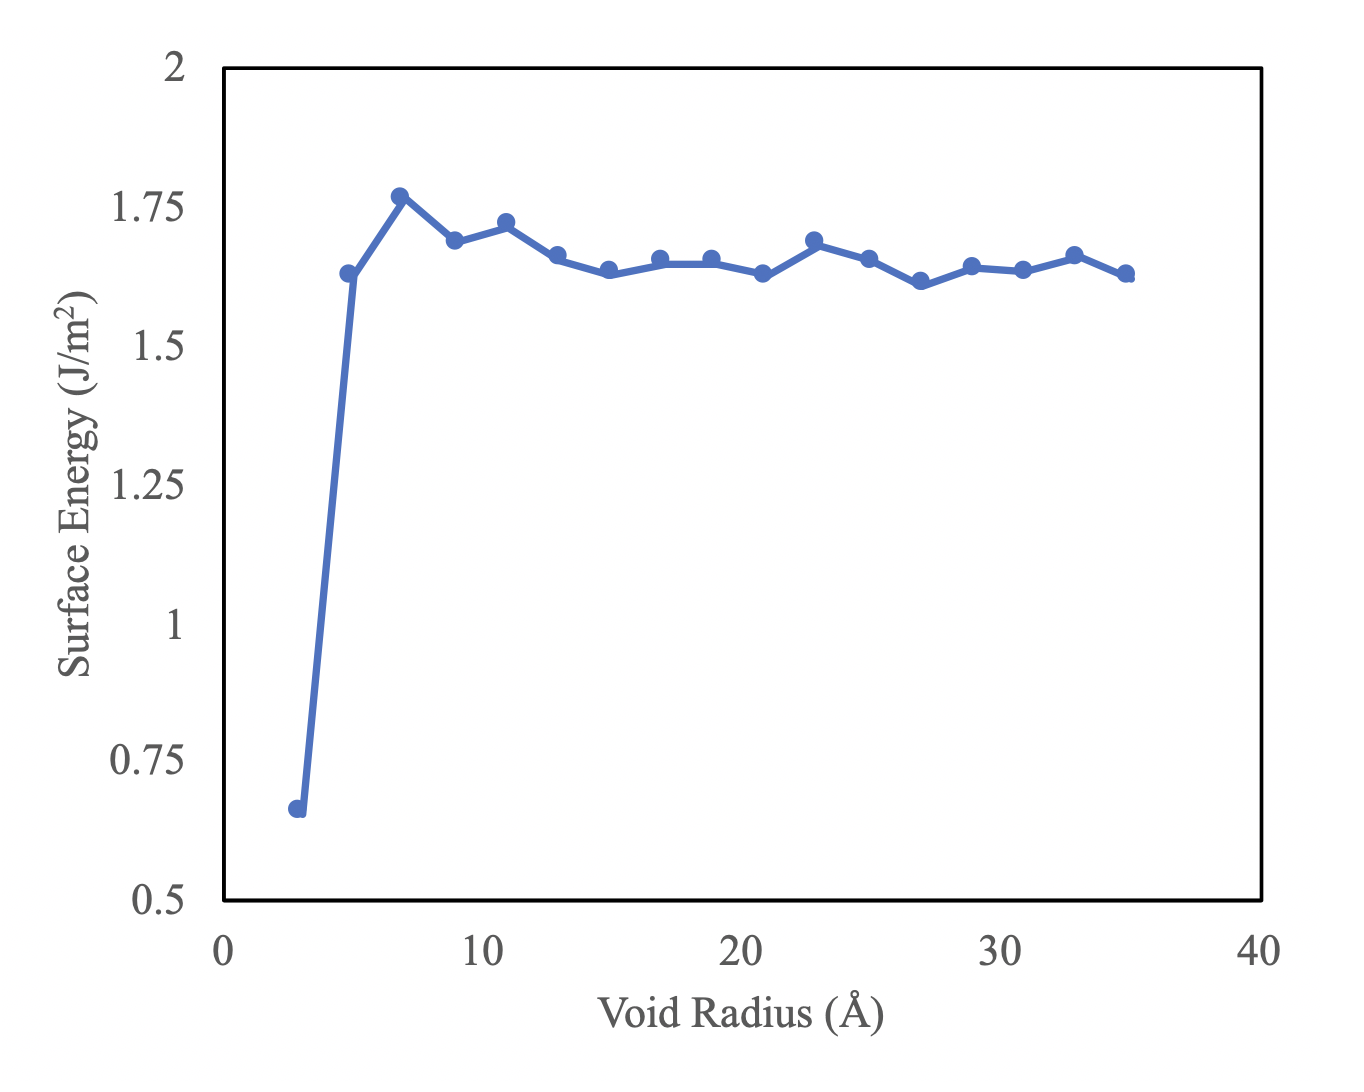
\includegraphics[width=0.6\textwidth]{6_size}
\end{center}
\caption{The void surface energy as a function of void radius for a U-10Zr alloy at 1000 K. }
\label{fig:size}
\end{figure}

An example void is shown in Fig. \ref{fig:void} for a U-10Zr alloy composition at 1200 K. The image is a slice through the three-dimensional supercell and the slice has a width of 10 \AA, allowing for the visualization of the void surface character. We are able to see the void maintains a spherical shape, while there does exist some surface roughening and local reorientation of atoms. The associated void surface energy for all temperatures and compositions is shown in Fig. \ref{fig:Esurf}. The surface energy increases as a function of Zr content, with a total increase of approximately 0.8 J/m$^2$ for $\gamma$U-Zr at 1000 K moving from bcc U to bcc Zr. The variation with temperature depends on the composition, with more variation observed with less Zr. There is no statistically significant difference in the surface energy as a function of temperature for compositions above 50 atomic percent Zr, but there is an increase of up to 0.2 J/m$^2$ for low Zr alloys. This is very similar to the trends observed for surface energies in U-Mo alloys \cite{beelerumo}. It should be noted that although bulk system values are presented in section \ref{sec:res1} for systems at 1400 K, they are not presented here. This is due to the systems being very near the melting point, which is approximately 1400 K for $\gamma$U, and the effect of a void further destabilizing the crystal and inducing melting. Thus, no results for surface energies at 1400 K are reported. 

\begin{figure}[!htp]
\begin{center}
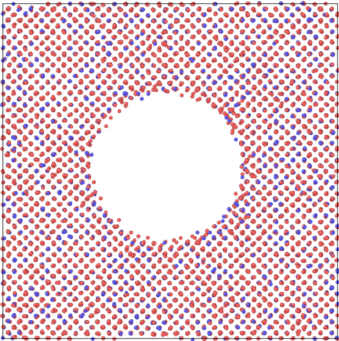
\includegraphics[width=0.6\textwidth]{7_void}
\end{center}
\caption{An example void in U-10Zr at 1200 K. The void is approximately 5 nm in diameter. }
\label{fig:void}
\end{figure}

\begin{figure}[!htp]
\begin{center}
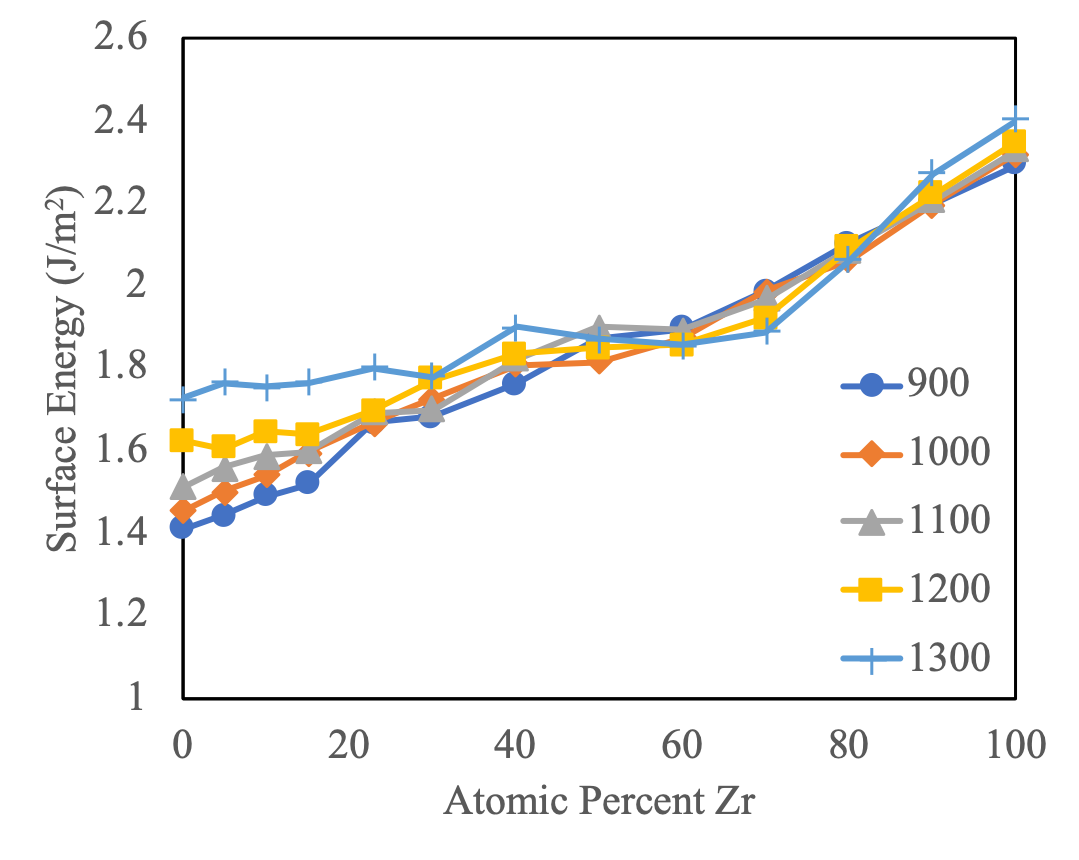
\includegraphics[width=0.6\textwidth]{8_Esurf}
\end{center}
\caption{Surface energy as a function of atomic percent Zr for temperatures from 900 K up to 1300 K.}
\label{fig:Esurf}
\end{figure}

\FloatBarrier

For the determination of the change in the free energy of a void with increasing temperature, a single composition was emphasized, that of U-10Zr (approximately 23 atomic percent), as this is the primary alloy composition of historical and future relevance. The calculation of the surface energy was refined from a temperature perspective, in that increments of 25 K, instead of 100 K, were utilized. Additionally, the temperature range was extended down to 800 K. Finally, the number of simulations for each individual system was increased from 5 to 50, to refine the accuracy of the dataset. The refined surface energy (eq. \ref{eq:surface} as a function of temperature and the change in entropy \ref{eq:entropy_alt} as a function of temperature are shown in Fig. \ref{fig:u23void}. The surface energy increases with increasing temperature, from approximately 1.6 J/m$^2$ at 800 K to 1.75 J/m$^2$ at 1300 K. This leads to a positive entropy increase with increasing temperature. The change in entropy is zero at 800 K as this is taken as our point of reference for this system. The data for this system is somewhat noisy, due to both temperature and compositional effects, in spite of efforts to increase the statistical certainty by increasing the sample size. 
\begin{figure}[!htp]
\begin{center}
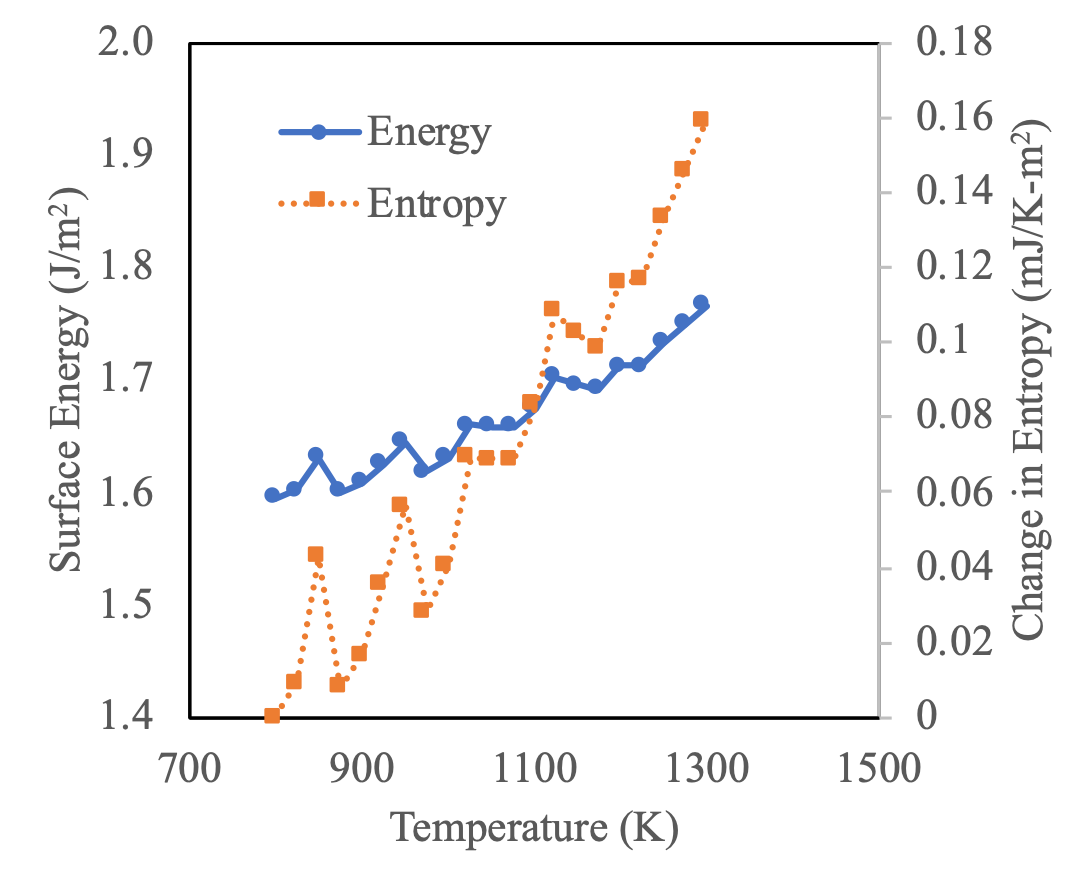
\includegraphics[width=0.6\textwidth]{9_u23void}
\end{center}
\caption{Change in the surface energy and entropy as a function of temperature in $\gamma$U-10Zr.}
\label{fig:u23void}
\end{figure}

The subsequent surface free energy as a function of temperature is shown in Fig. \ref{fig:free}.  Due to the increasing entropy, a trend can be seen pointing towards a slight decrease in free energy with increasing temperature. This indeed makes qualitative sense, in that the free energy decreases with increasing temperature due to entropic contributions. This shows that in spite of the surface energy increasing slightly with temperature, entropic effects become more prevalent at higher temperatures and lead to a decrease the magnitude of the surface free energy. To make this approximation of the magnitude of the surface free energy, we must make an assumption regarding our system. Since we are unable to calculate data down to 0 K (due to the predicted instability of the $\gamma$ phase at low temperature) where entropic effects are negligible, we must identify a point where we \textit{assume} entropic effects are negligible. We take this point to be the lowest temperature investigated in the data set, 800 K. In reality, there likely are entropic effects at 800 K, but also likely is that these effects are substantially smaller than any effects at temperatures greater than 1000 K. That the free energy change between 800 K and 1000 K is quite small serves to substantiate our approximation. 

\begin{figure}[!htp]
\begin{center}
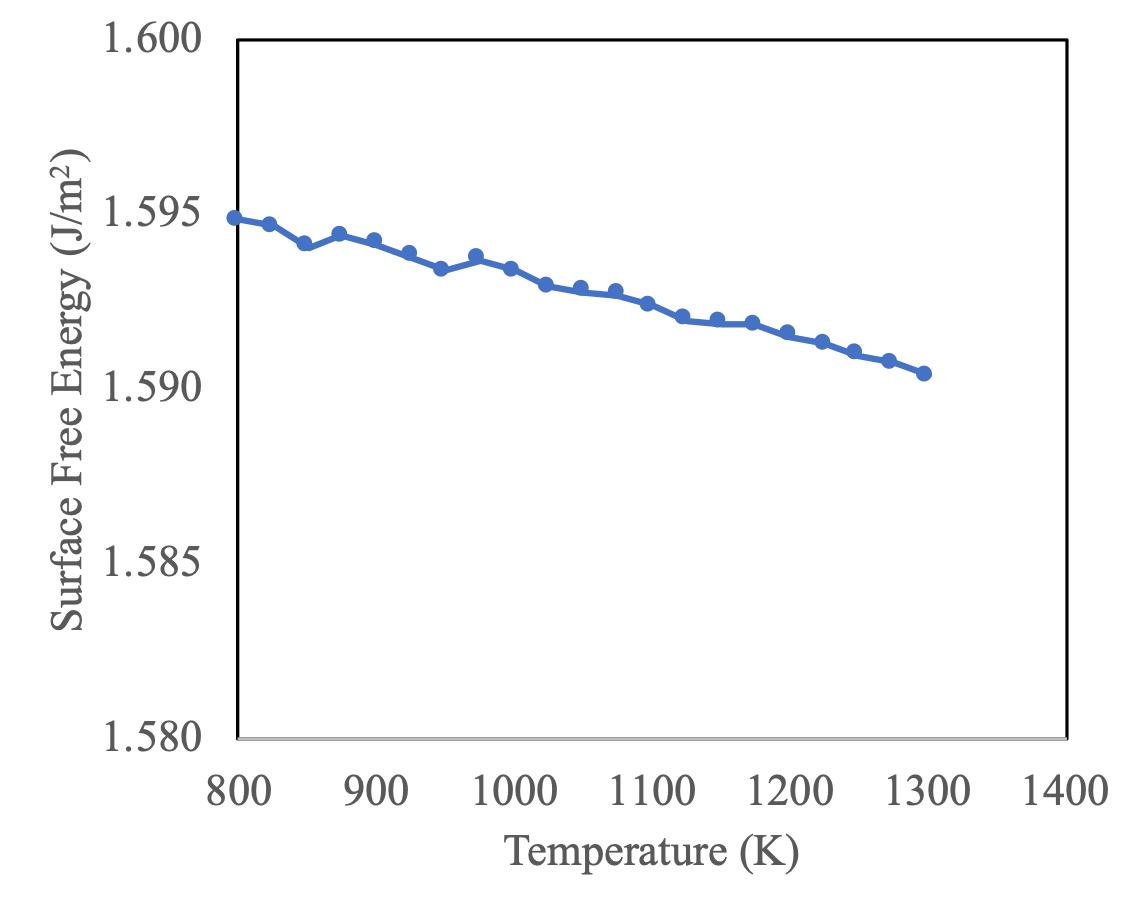
\includegraphics[width=0.6\textwidth]{10_free}
\end{center}
\caption{The surface free energy as a function of temperature in $\gamma$U-10Zr.}
\label{fig:free}
\end{figure}

\FloatBarrier

\subsection{Atomistically informed fuel performance simulations}

BISON is a finite element based fuel performance code built on the MOOSE framework \cite{tonks2017}, capable of describing swelling of metallic fuel systems. One of the available fuel swelling models for U-Zr was originally presented in \cite{olander76}. The total gaseous swelling is a function of the radius and number density of fission gas bubbles:

\begin{equation}
  \left(\frac{\Delta V}{V_0}\right)_{g}=\frac{4\pi}{3}R^3 N
  \label{eq:swelling}
\end{equation} where \textit{R} is the radius of bubbles and \textit{N} is the number density. The radius is determined by:

\begin{equation}
  \label{bubble_radius}
  R = \sqrt{\frac{3 k_B T Y_{gas} \dot{F} t}{4 \pi 2 \gamma N}},
\end{equation} where $k_B$ is the Boltzmann constant, $T$ is the temperature (K), $\gamma$ is the surface tension of the fuel (J/m$^2$) \cite{karahan2009}, $Y_{gas}=0.3017$ is the gaseous fission product yield, $\dot{F}$ is the fission rate density, $t$ is time, and $N$ is the number density of bubbles. The fuel is assumed to exhibit a constant number density of bubbles that grow as a function of burnup and the bubbles are assumed to be in mechanical equilibrium with the solid \cite{olander76}. The porosity of the system is directly related to the gaseous swelling: 

\begin{equation}
  p_{gas} = \frac{\left(\frac{\Delta V}{V_0}\right)_{g}}{1 + \left(\frac{\Delta V}{V_0}\right)_{g}},
\end{equation}

From these equations, it can be seen that the gaseous swelling is proportional to $\gamma^{-3/2}$. The only previously reported value of the surface energy in U-Zr fuels was 0.8 J/m$^2$ \cite{tsuboi1992} (although it was not clear how this value was determined). From the above molecular dynamics investigations, with the assumption that surface tension and surface energy are equal, it was shown that the surface tension is actually significantly higher than 0.8 J/m$^2$. As such, an example investigation of the effect of surface tension on fission gas swelling was undertaken. In Fig. \ref{fig:plot_porosity_var_gamma}, the porosity as a function of burnup at three unique surface tensions is shown. An increase in the surface tension depresses the rate of porosity accumulation, which in turn delays fission gas release. Physically, this is because higher surface tension causes the gas within each bubble to be compressed to a higher pressure, and the same number of gas atoms is contained in a smaller volume, which in turn delays the interconnection of bubbles and subsequent fission gas release. Given that a primary factor in fuel pin failure is plenum pressure, which is directly related to fission gas release, obtaining accurate porosity accumulation is critical in predicting accurate fuel evolution under operation. The refinement of fundamental materials properties via atomistic simulations has reduced the inherent uncertainty in the fuel performance simulations and provided a basis for further investigation of key properties. 

\begin{figure}[!htp]
\begin{center}
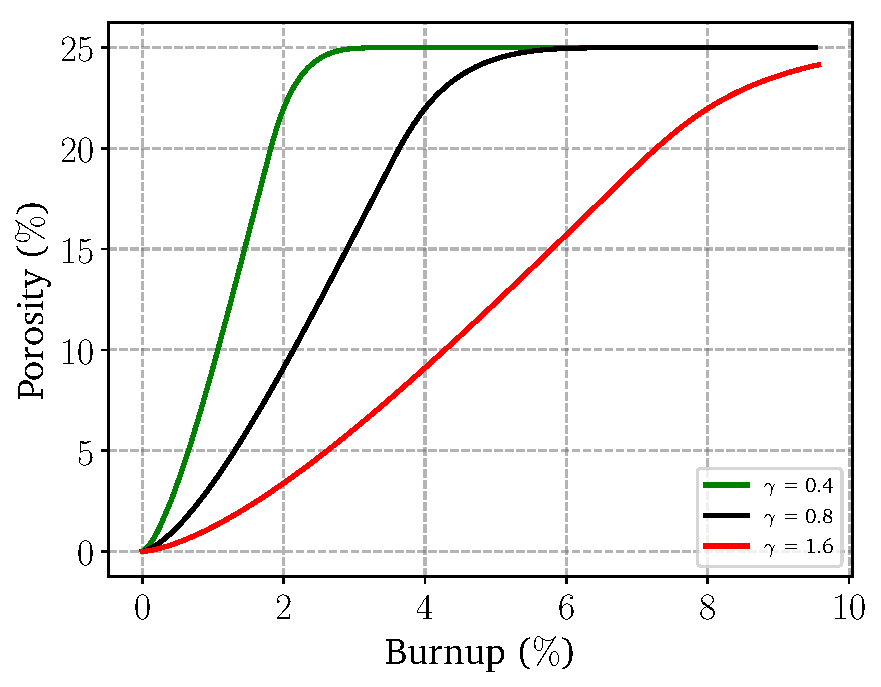
\includegraphics[keepaspectratio, width=4.0in]{11_plot_porosity_var_gamma}
\end{center}
\caption{Comparison of porosity as a function of burnup for three different values of the fuel surface tension.}
\label{fig:plot_porosity_var_gamma}
\end{figure}

\FloatBarrier

\section{Conclusions}

In this work, molecular dynamics simulations were utilized to investigate a number of bulk thermophysical properties in $\gamma$U-Zr, demonstrating impressive agreement with experiment for both thermal expansion and heat capacity, while providing a much more broad scope of data with respect to temperature and composition than previously existed in the literature. The void surface energy as a function of radius, temperature and composition was determined, indicating a value of approximately 1.7 J/m$^2$ for U-10Zr in the temperature regime of interest. Entropic effects were included to analyze the void free energy as a function of temperature, which leads to a slight decrease in the free energy with increasing temperature. Finally, fuel performance simulations were performed to investigate the effect of surface energy on the porosity accumulation as a function of burnup, showing that an increase in the surface energy decreases the rate of fission gas swelling in metallic fuels. 

This work provided a more expansive investigation into a number of critical properties as a function of both temperature and composition than is currently present within the literature. This work also provided the first study of any kind into the surface energy of U-Zr alloys. Additionally, the refinement of fundamental materials properties via atomistic simulations has reduced the inherent uncertainty in fuel performance simulations and provided a basis for further investigation of key properties.


\section{Acknowledgement}
This work is supported by the U.S. Department of Energy, Office of Nuclear Energy, Nuclear Energy Advanced Modeling and Simulation (NEAMS) Program. This manuscript has been authored by Battelle Energy Alliance, LLC under Contract No. DEAC07-05ID14517 with the U.S. Department of Energy. The United States Government retains and the publisher, by accepting the article for publication, acknowledges that the United States Government retains a nonexclusive, paid-up, irrevocable, world-wide license to publish or reproduce the published form of this manuscript, or allow others to do so, for United States Government purposes. This research made use of the resources of the High Performance Computing Center at Idaho National Laboratory, which is supported by the Office of Nuclear Energy of the U.S. Department of Energy and the Nuclear Science User Facilities under Contract No. DE-AC07-05ID14517.



\bibliography{MARMOTbib}


\end{document} 
